
Vzhledem k vysokému počtu dat pro jeden kalendářní rok %doplnit pocet radku!!!
, jsem se rozhodla provést analýzu na měsíčním výběru dat z tohoto období. Jako zkoumaný měsíc jsem vybrala měsíc říjen, neboť v tomto měsíci bylo v databázi evidováno přes dva a půl milionu pozorování, což je nejvíce ze všech měsíců v roce 2022.  %overit!!!.
Zároveň v porovnání s letními měsíci a Vánocemi se v říjnu nevyskytují významné sezónní výkyvy.

Zkoumaná říjnová data obsahují $2 634 614$ řádků a patnáct sloupců. Každý řádek odpovídá jednomu záznamu v databázi shrinku daného produktu. Sledované údaje ve sloupcích jsou následovné, 
% \subsubsection{Sledované údaje}
\begin{itemize}
    \item id prodejny, kategorická proměnná,
    \item id produktu, kategorická proměnná,
    \item datum transakce, kategorická proměnná,
    \item typ shrinku, kategorická proměnná,
    \item L1, kategorická proměnná,
    \item L2, kategorická proměnná,
    \item L4, kategorická proměnná,
    \item L5, kategorická proměnná,
    \item L6, kategorická proměnná,
    \item expirace, kategorická proměnná,
    \item množství, spojitá proměnná,
    \item ztracená nákladová cena, spojitá proměnná,
    \item den v týdnu, kategorická proměnná,
    \item číslo den, kategorická proměnná,
    \item období v měsíci (rozdělení měsíce na pět částí), kategorická proměnná,
\end{itemize}
Původní sloupec datum jsem rozdělila na tři jiné proměnné, a to den v týdnu, číslo dne a období v měsíci a sloupec datum jsem vynechala. Z důvodu vysokého počtu záznamů a odlišné povahy dvou typů shrinků jsem data dále rozdělila na shrinky typu damages a shrinky typu inventory. 


\subsection*{Damages shrinky}
Následující část text bude věnována rozboru dat pro shrinky typu damages.

\subsubsection{Výběr dat}
% výběr dle zastoupení shrinků a kategorií produktů a dle outlierů.

Nejprve jsem graficky analyzovala zastoupení shrinků v závislosti na vybraných proměnných pomocí nástroje Power BI, viz obr. \ref*{obr:rok:g:zastoupeni1}. V návaznosti na zjištěné zastoupení shrinků v datech jsem se rozhodla vybrat pouze ty typy shrinků, které tvoří více jak jedno procento z celkových nákladů (tj. náklady činily alespoň jeden milion korun). Vynechala jsem tedy shrinky s označením 25, 28, 31, 32, 34 a naopak shrinky 3,4,6,8,64 byly ponechány. Obdobně jsem přistupovala k záznamům i z hlediska kategorie produktu úrovně L1, jelikož z grafu je patrné, že majoritní zastoupení mají pouze dvě kategorie, a to kategorie superfresh a fresh produktů. Všechny záznamy se zbylymi kategoriemi (HBC, others, nonfood, dry food a tobacco) jsem z datasetu odstranila. Těmito kroky jsem zredukovala původní počet řádků datasetu z $1 497 485$ na $1 393 223$ řádků.

\begin{figure}[hbtp!]
    \centering
    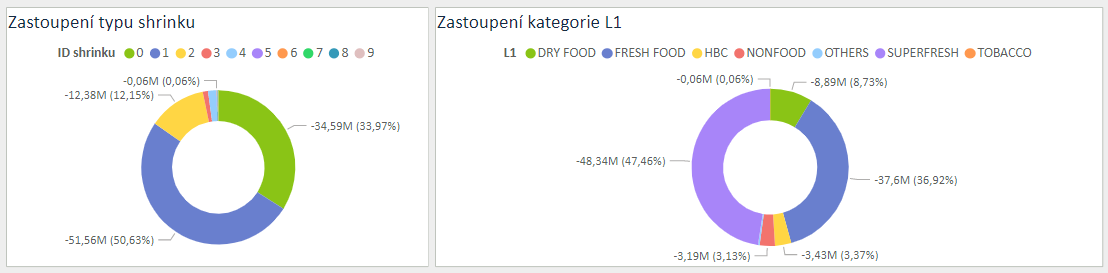
\includegraphics[width=\textwidth]{obrazky/grafy/zastoupeni1.png}
    \caption{Zastoupení shrinků typu damage a zastoupení kategorie L1 v datech z října roku 2022.}
    \label{obr:rok:g:zastoupeni1}
\end{figure}

Jako cílové sloupce (target sloupec) jsem určila sloupec s typem shrinku, množství produktu a nákladovou cenu. Zbylých jedenáct sloupců slouží jako vysvětlující proměnné, dále budou označovány jako příznaky, pro cílový sloupec. Všechny vybrané příznaky jsou kategorické proměnné, které lze dále rozdělit na nominální a ordinální. Nominální proměnné jsou id prodejny, id produktu, kategorie L1, L2, L4, L5 a L6. Ordinální expirace, den v týdnu, číslo dne a období měsíce.

Target hodnotu pro cílový sloupec typu shrinku jsem přeznačila na hodnoty od nuly do $n_p$, kde $n_p$ je počet kategorií v $p$-tém příznaku. Pro další výpočty bylo vhodné přesunout se z nominálních kategorických hodnot na číselné hodnoty. Pro tyto účely jsem zvolila metodu \emph{target encoding} %!!! odkaz do teorie, princip meotdy je vysvětlený v kapitole...

Dále jsem se zabývala identifikací odlehlých hodnot. Nejprve jsem vizualizovala hodnoty pomocí grafu, obrázky \ref*{obr:rok:g:outlierN} a \ref*{obr:rok:g:outlierO}. % !!! jakeho grafu 

\begin{figure}[hbtp!]
    \centering
    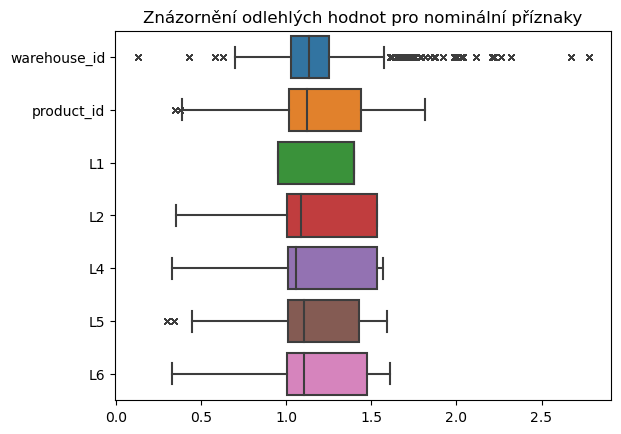
\includegraphics[width=.5\textwidth]{obrazky/zntb/box_nominal.png}
    \caption{Znázornění odlehlých hodnot pro nominální příznaky.}
    \label{obr:rok:g:outlierN}
\end{figure}
\begin{figure}[hbtp!]
    \centering
    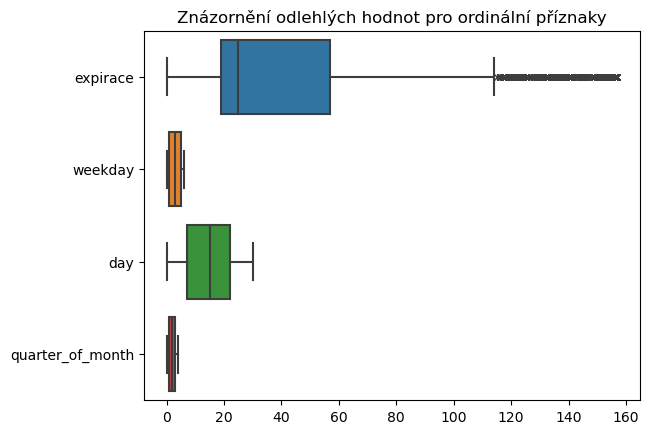
\includegraphics[width=.5\textwidth]{obrazky/zntb/box_ordinal.png}
    \caption{Znázornění odlehlých hodnot pro nominální příznaky.}
    \label{obr:rok:g:outlierO}
\end{figure}

Pomocí Tukeyho testu jsem identifikovala přes $150 000$ outlierů pro příznak id prodejny (\texttt{warehouse\_id}), čímž se dataset zredukoval na $1 218 453$ řádků.

V dalším kroku jsem se zaměřila na míru korelace mezi proměnnými. Vizualizovala jsem data pomocí scatter matice pro všechny proměnné, matice je možné vidět na obr. č. \ref*{obr:nb:scatter}.

\begin{figure}[hbtp!]
    \centering
    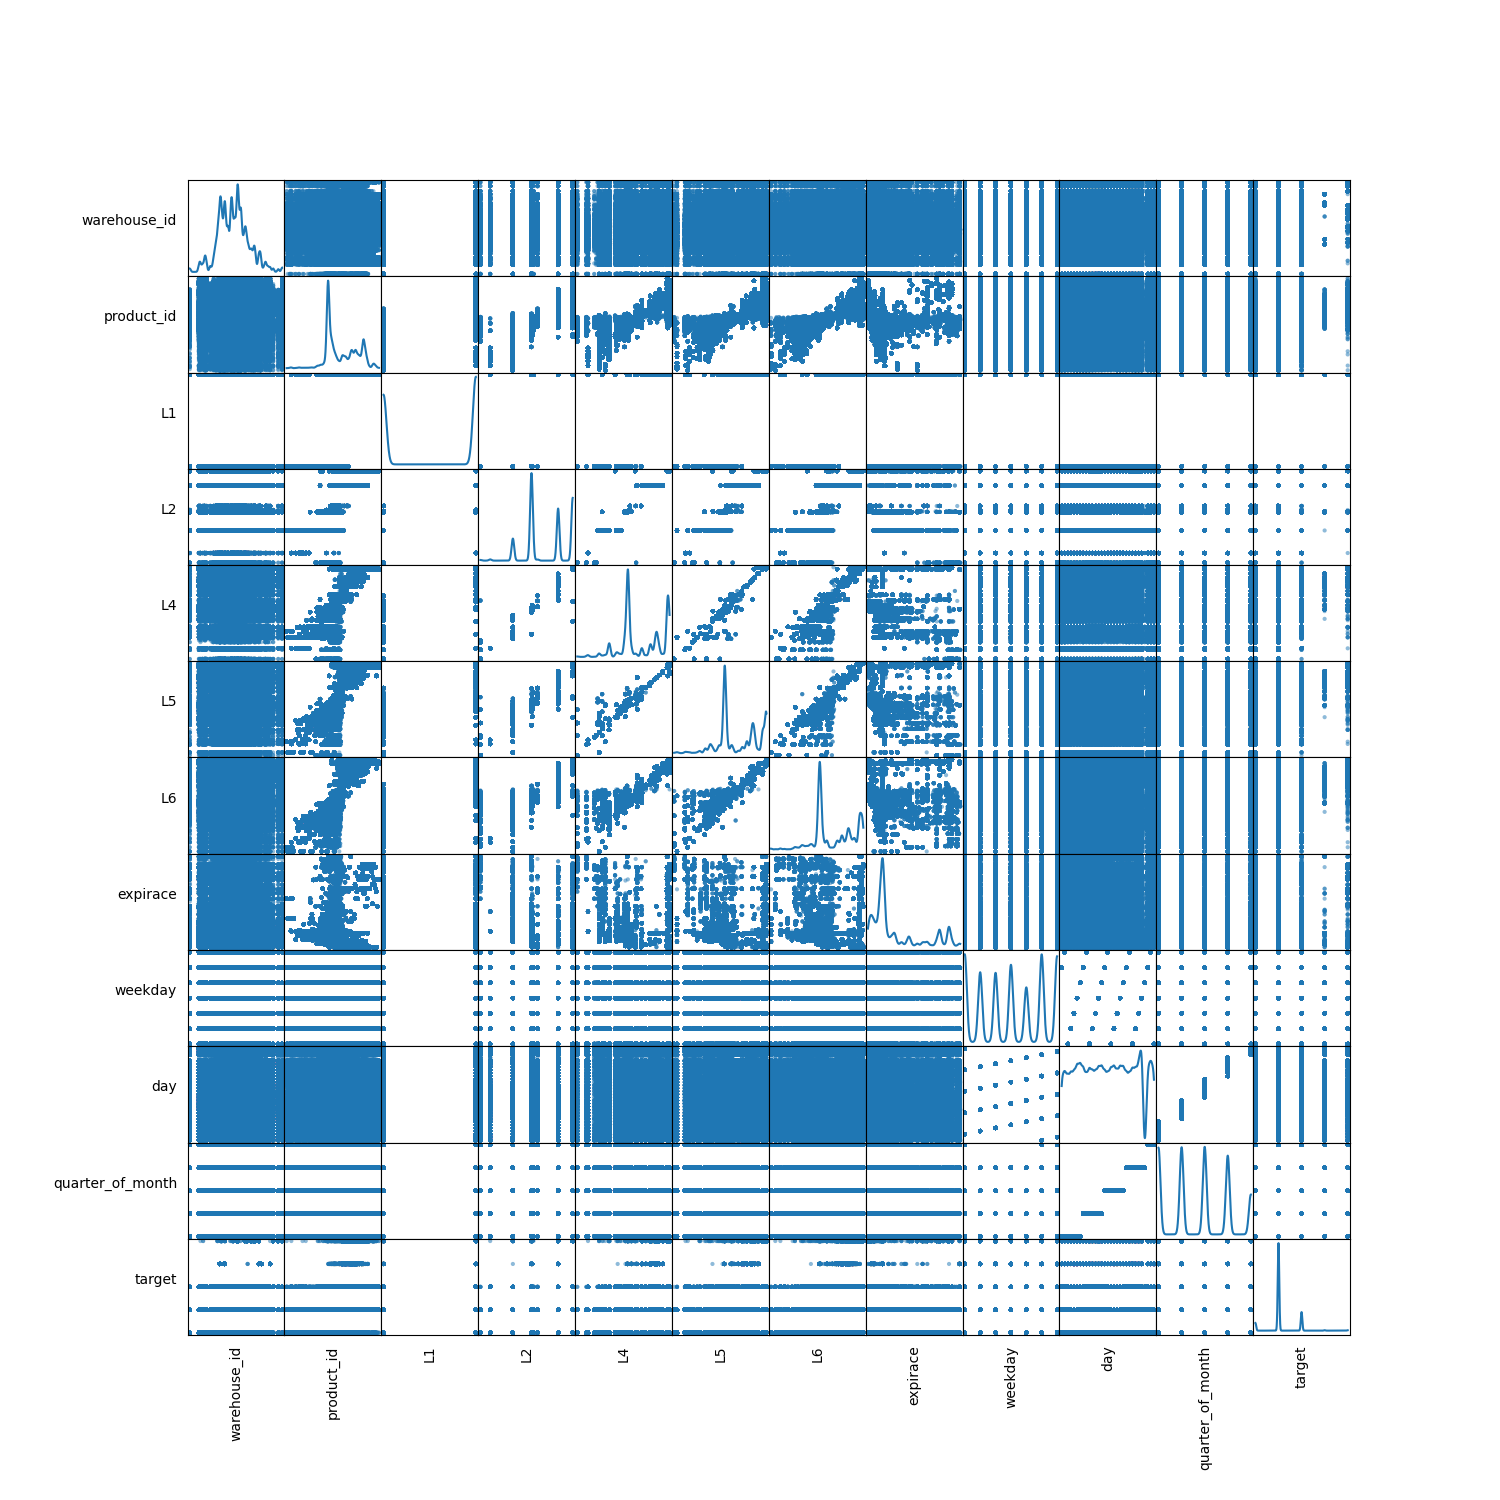
\includegraphics[width=.6\textwidth]{obrazky/zntb/MyScatter.png}
    \caption{Scatter matice příznaků.}
    \label{obr:nb:scatter}
\end{figure}
 
Jako první jsem zvolila $\chi^2$ test. Vzhledem k vysokému počtu dat je matice příliš řídká, a proto nejsou výsledné hodnoty odpovídající a test je tedy pro tuto úlohu nespolehlivý.
Jiným měřítkem pro korelaci mezi proměnnými je Pearsonův korelační koeficient.

Výslednou matici popisující korelační vztahy mezi příznaky jsme vizualizovala teplotní mapou, která je zobrazena na obrázku \ref*{obr:nb:pearson}. Z výsledků je patrné, že mezi jednotlivými kategoriemi produktů a produkty je silná korelace. Toto zjištění je zcela logické neboť jse jedná o stromovou strukturu kategorií. Zároveň existuje korelace mezi produktovými kategoriemi a expirací produktu. 

\begin{figure}[hbtp!]
    \centering
    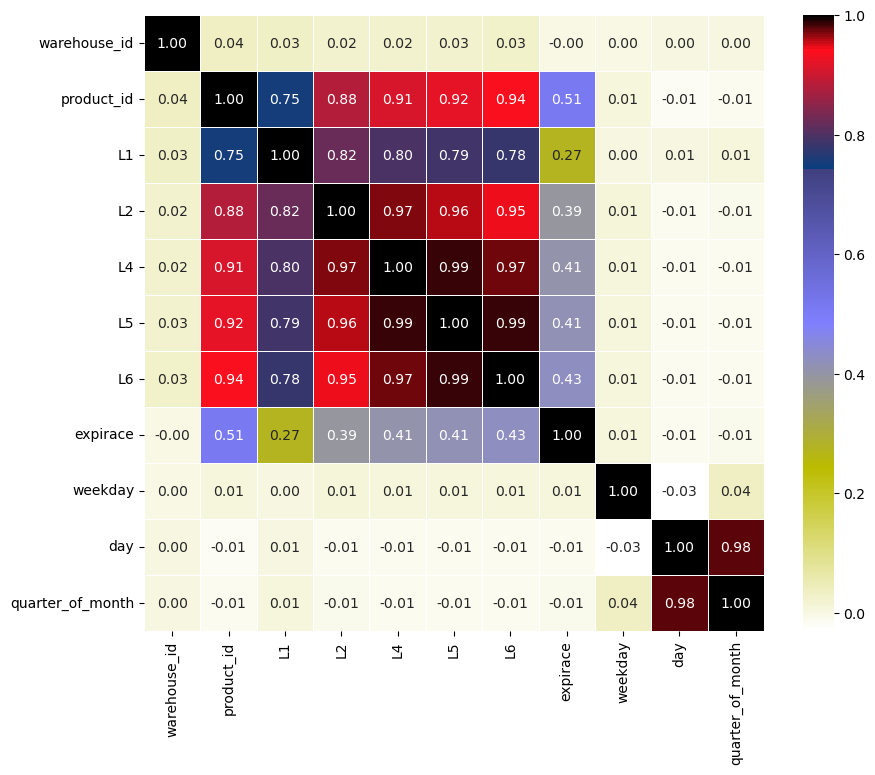
\includegraphics[width=.8\textwidth]{obrazky/zntb/pearson.png}
    \caption{Matice korelačních koeficientů mezi příznaky.}
    \label{obr:nb:pearson}
\end{figure}

Dále jsem použila výpočet koeficientů vzájemná informace \footnote{\emph{mutual information}}, která určuje kolik informace sdílí dvě proměnné. % !!!zdroj
Matice vypočítaných koeficientů je na obr.\ref*{obr:nb:MI}.

\begin{figure}[hbtp!]
    \centering
    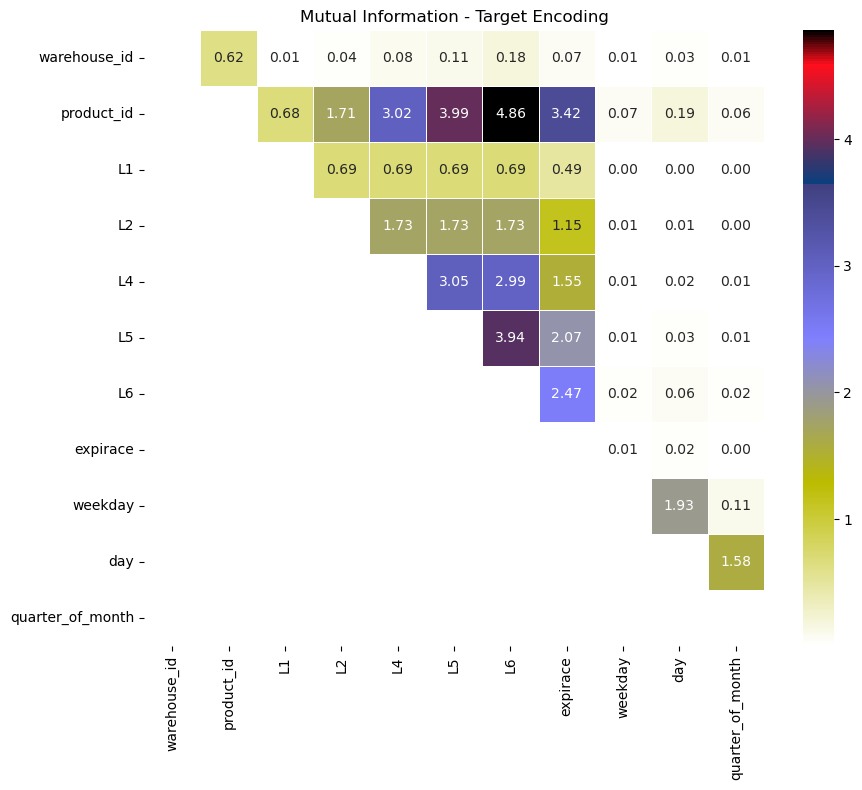
\includegraphics[width=.8\textwidth]{obrazky/zntb/MI_TE.png}
    \caption{Matice koeficientů vzájemná informace mezi příznaky.}
    \label{obr:nb:MI}
\end{figure}

Opět pro znázornění závislosti mezi proměnnými jsem použila koeficient Cramers V a Thiels U. %!!! dopsat co to je %!!!zdroj, odkaz na teorii

\begin{figure}[hbtp!]
    \centering
    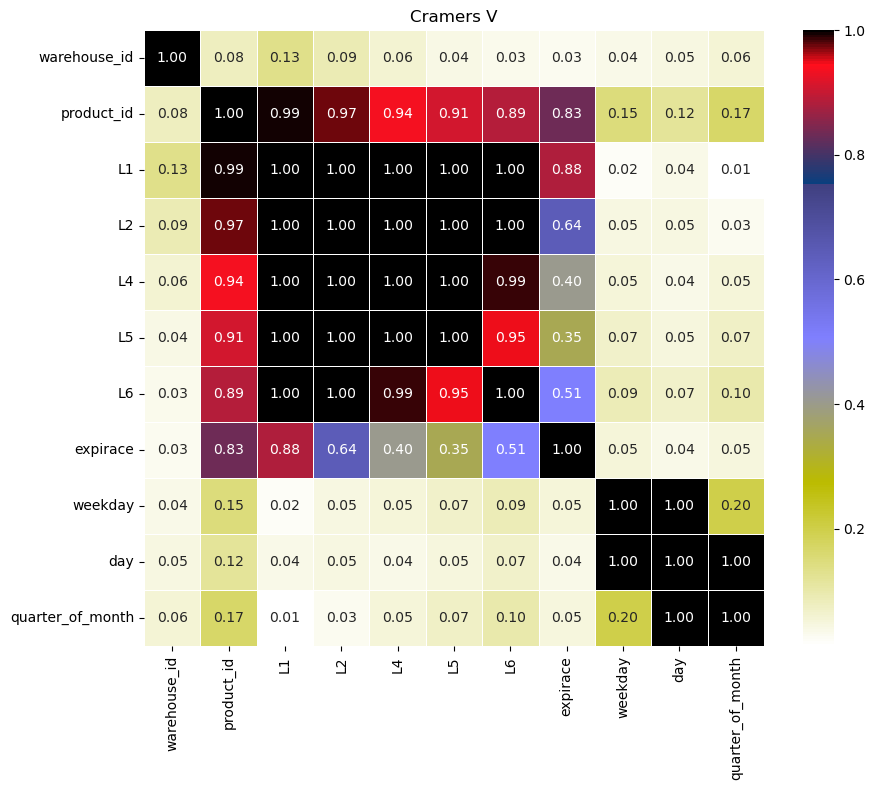
\includegraphics[width=.8\textwidth]{obrazky/zntb/cramers_u.png}
    \caption{Matice koeficientů Cramers U mezi příznaky.}
    \label{obr:nb:cramers}
\end{figure}

\begin{figure}[hbtp!]
    \centering
    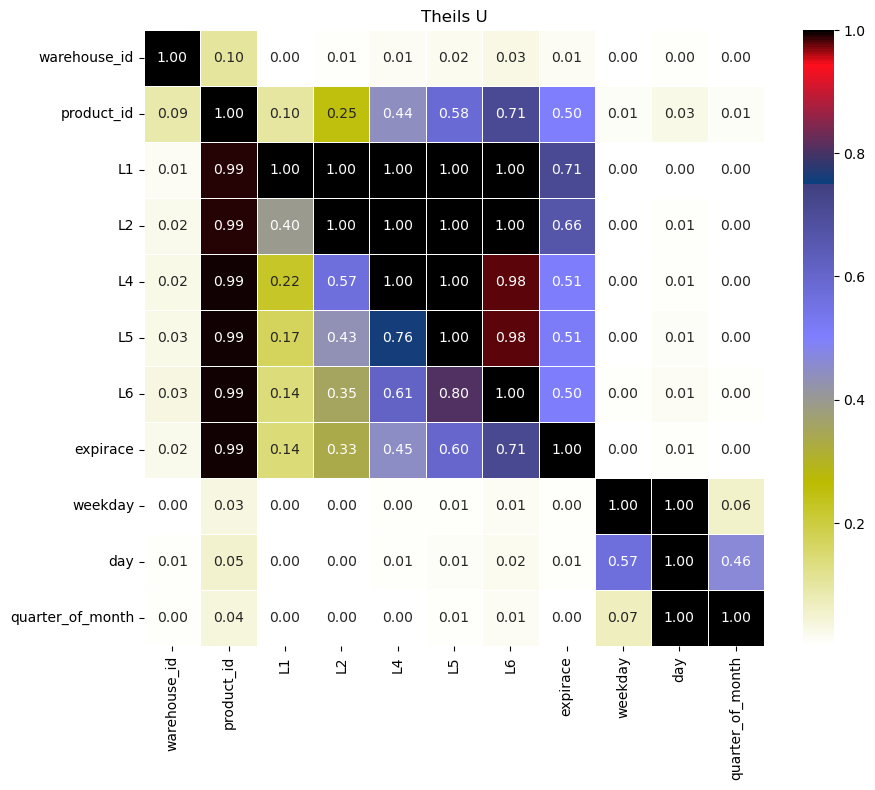
\includegraphics[width=.8\textwidth]{obrazky/zntb/theils_u.png}
    \caption{Matice koeficientů Thiels V mezi příznaky.}
    \label{obr:nb:thiels}
\end{figure}

V dalším testu jsem otestovala multikolinearitu dat pomocí rozptylového inflačního faktoru (VIF). Jako hraniční faktor jsem zvolila hodnotu 40 VIF. Čímž došlo k redukci příznaků z jedenácti na pět na kategorii L1, číslo dne, období měsíce, id prodejny a den v týdnu.

\begin{figure}
    \centering
    \begin{minipage}{.5\textwidth}
      \centering
      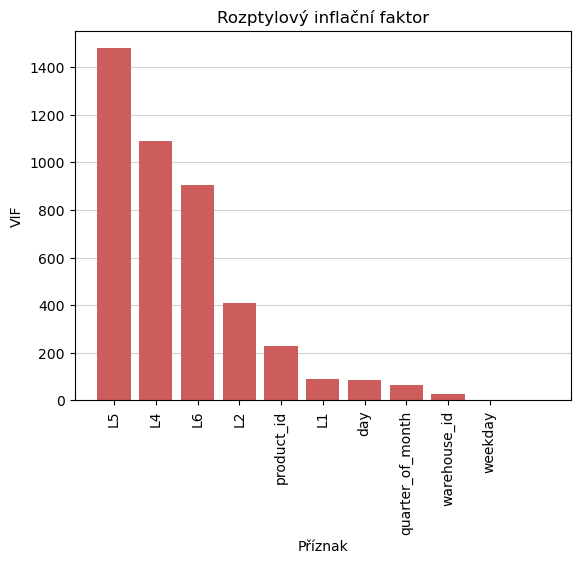
\includegraphics[width=.8\textwidth]{obrazky/zntb/VIF.png}
      \caption{Rozptylový inflační faktor.}
      \label{obr:nb:vif}
    \end{minipage}%
    \begin{minipage}{.5\textwidth}
      \centering
      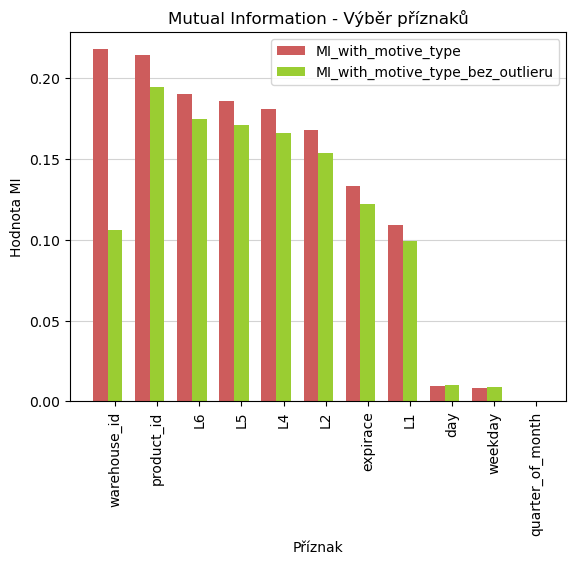
\includegraphics[width=.8\textwidth]{obrazky/zntb/MI_feature_selection.png}
      \caption{Matice koeficientů vzájemná informace mezi příznaky a cílovým sloupcem typ shrinku.}
      \label{obr:nb:MI_FS}
    \end{minipage}
    \end{figure}


Jako další metodu po výběr příznaků jsem vypočítala hodnotu koeficientů vzájemné informace mezi všemi příznaky s target sloupcem. Na obrázku \ref*{obr:nb:MI_FS} lze vidět jak hodnotu jednotlivé proměnné souvisí s cílovým sloupcem.

Potom jsem aplikovala na data analýzu hlavních komponent \ref*{obr:nb:pca_roztyl_komponetn}. Na obrázcích \ref*{obr:nb:pca_roztyl_komponetn} a \ref*{obr:nb:pca_kum_roztyl_komponetn} jsou znázorněny prvních deset komponent a rozptyl který v datech vysvětlují. Na základě hodnot jsem vybrala prvních pět komponent, poté jsem vypočítala příspěvky příznaků k těmto komponentám a vybrala jsem ty příznaky, které příspívají nejvíce - to jsou příznaky id prodejny, den v týdnu, expirace, den a období v měsíci.

\begin{figure}
    \centering
    \begin{minipage}{.5\textwidth}
      \centering
      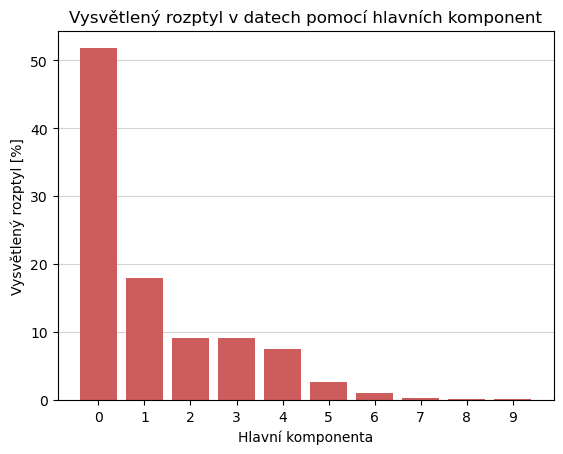
\includegraphics[width=.8\textwidth]{obrazky/zntb/pca-roztyl_komponetn.png}
      \caption{PCA - vysvětlený rozptyl hlavních komponent.}
      \label{obr:nb:pca_roztyl_komponetn}
    \end{minipage}%
    \begin{minipage}{.5\textwidth}
      \centering
      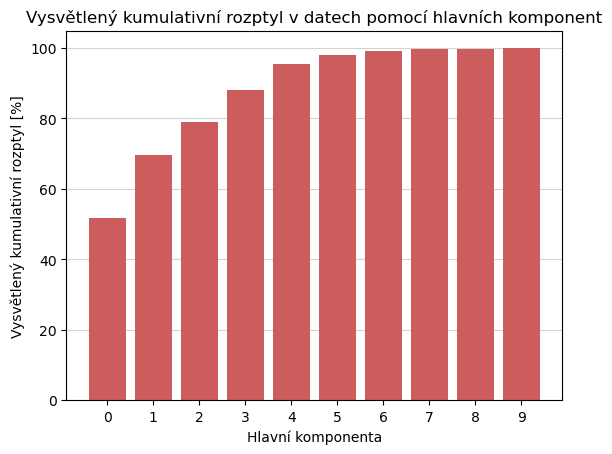
\includegraphics[width=.8\textwidth]{obrazky/zntb/pca-kum_roztyl_komponetn.png}
      \caption{PCA - kumulativní vysvětlený rozptyl hlavních komponent.}
      \label{obr:nb:pca_kum_roztyl_komponetn}
    \end{minipage}
    \end{figure}

\begin{figure}[hbtp!]
    \centering
    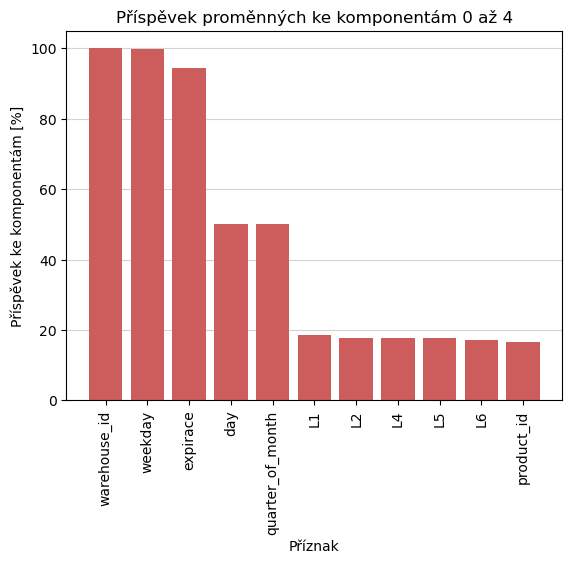
\includegraphics[width=.8\textwidth]{obrazky/zntb/pca-prispevky.png}
    \caption{Příspěvek proměnných ke komponentám 0 až 4.}
    \label{obr:nb:pca_prispevek}
\end{figure}
    